
\subsection{Definition}

A \textbf{branch-and-bound} algorithm consists of a systematic enumeration of
candidate solutions by means of state space search: the set of candidate
solutions is thought of as forming a rooted tree with the full set at the root.

\begin{itemize}
    \item Explores branches of this tree, which represent subsets of the
solution set. 
    \item Note that before enumerating the candidate solutions of a branch, the
branch is checked against upper and lower estimated bounds on the optimal
solution, and is discarded if it cannot produce a better solution than the best
one found so far by the algorithm.
\end{itemize}

\subsection{Solving the knapsack problem with B\&B}

Given the following knapsack problem :
    \begin{tabular}{cl}
        maximize & $28x_1+30x_2 +20x_3$\\
        subject to & $4x_1+6x_2 +4x_3 \leq 9$\\
                   & $x_i \in \{0, 1\} \forall i$
    \end{tabular}

\subsubsection{Relaxation}
We can choose to relax in order to reduce the search space as much as possible.

\begin{enumerate}
    \item \textbf{Capacity relaxation}: Relax on the constraint by don't
        explore branch which already violated the constraint.

        $\Rightarrow$ Cut at tree branch when 
        we have surpassed the capacity.
        \begin{center}
        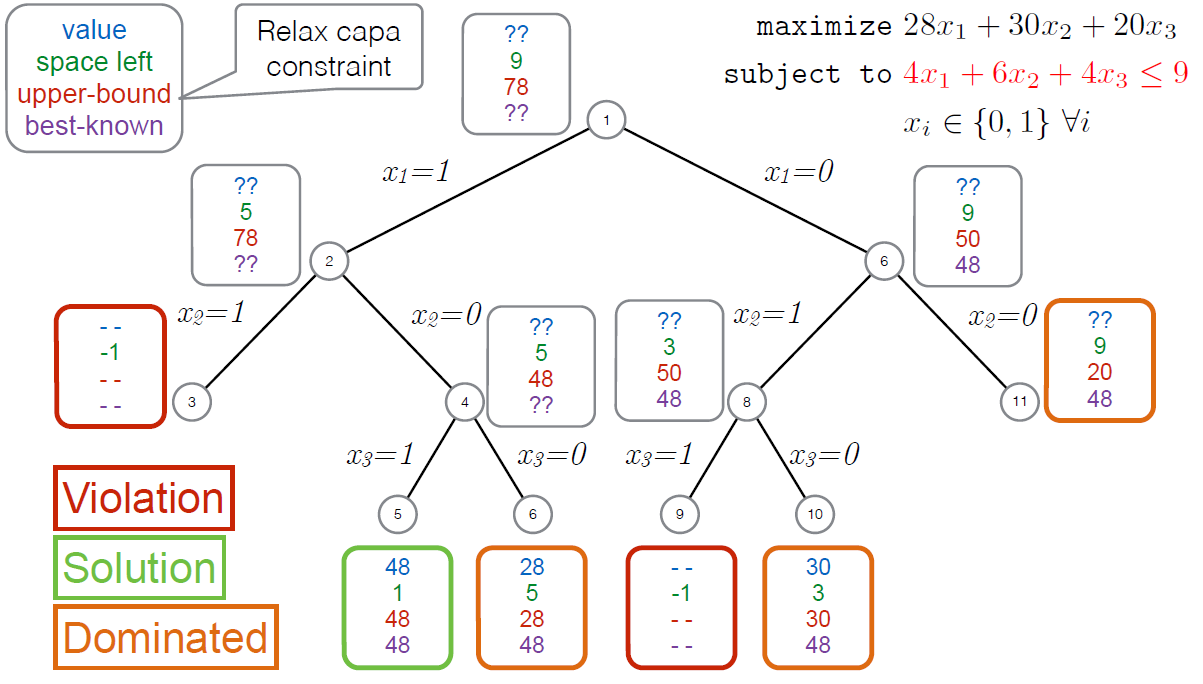
\includegraphics[width=12cm]{KnapsackBBCapaRelaxation.png}
        \end{center}
        It is far from optimal as our upper bound are not close enough to their real
        value.

    \item \textbf{Linear relaxation}: Relax on the value to maximize by
        calculating an upper bound and don't explore if the upper bound <
        actual best value.

        \paragraph{Upper bound computation}
        Given a set sorted by ratio $v_i/w_i$,
        \begin{eqnarray*}
            j &= min\{i \in I: \sum_{k \in 1,...,i} w_k > C\}\\
            UB &= \sum_{i<j} v_i + \frac{(C - \sum_{i \in 1..j-1} w_i)}{w_j} v_j
        \end{eqnarray*}

        $j$ is called the critical item which is in fact the first item (sorted by better ratio)
        which cannot be add entirely, so we just add the ratio of the item according to 
        the free space.

        \begin{center}
            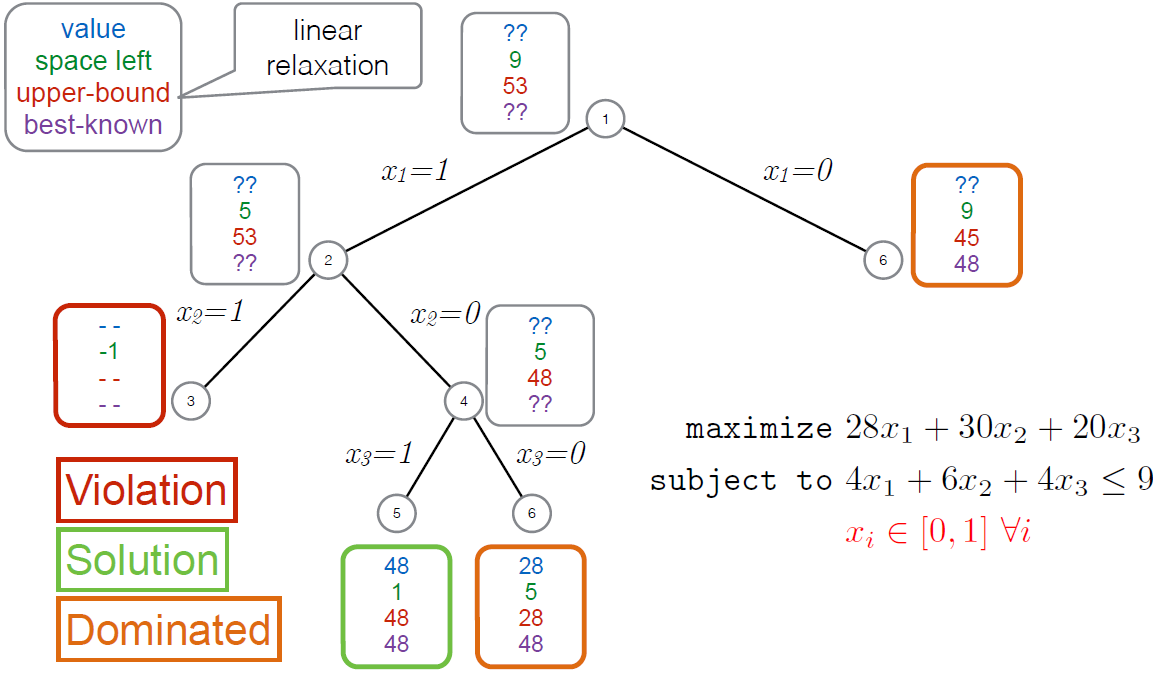
\includegraphics[width=12cm]{KnapsackBBLinearRelaxation.png}
        \end{center}

        Improving the precision of the upper-bound yields far better
        result. Take care however not to over/under estimate it (depending if you are
        on a maximisation or minimisation process) as it might prevent you to find the
        optimal solution.

\end{enumerate}


\subsection{B\&B pseudo-code}

\begin{tabular}{m{8cm}m{8cm}}
\begin{lstlisting}[mathescape, caption=BB with recursion]
def backtrackSearch(c) {
    if reject(P, c) then return
    if accept(P, c) then output(P, c)
    for s $\leftarrow$ children(c) do
        backtrackSearch(s)
}

backtrackSearch(root(P))
\end{lstlisting}
&
\begin{lstlisting}[mathescape, caption=BB with stack]
  def branchAndBound() = {
      var queue = List(root(P))

      while(queue.nonEmpty) {
          var c = queue.head
          queue = queue.tail

          if( ! reject(P, c)) {
            if( accept(P, c)) output(P, c)
            for (s $\leftarrow$ children(P, c))
            queue = s :: queue
          }
      }
  }
  \end{lstlisting}
\end{tabular}


\begin{itemize}
    \item For the knapsack, partial solution by a list of boolean: 
        $\begin{cases} 
            list[i]= 1 \text{ if item i is selected}\\
            list[i]= 0 \text{ else}\\
            \end{cases}$
        \end{itemize}



With the preceding algorithm, a partial solution will be represented as a growing vector
of zero and ones representing whether a given item as been selected or not.

\begin{figure}[!ht]
    \centering
    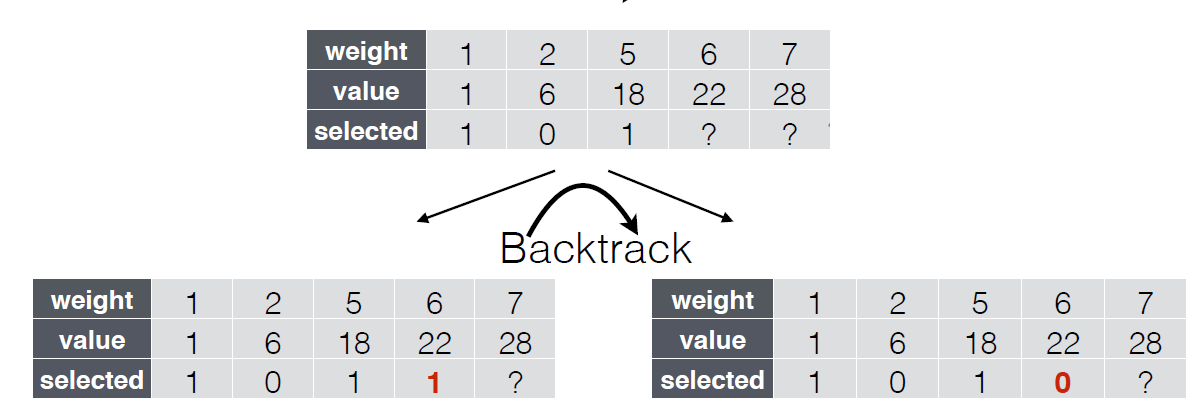
\includegraphics[width=\linewidth]{PartialSolBB.png}
    \label{fig:Knapsack_example}
\end{figure}
\FloatBarrier

This algorithm however has limitations, we must always evaluate the variables of the 
problem in the same order (We cannot affect $X_1$ then$ X_2$ at the left side of the tree 
while on the other side we affect $X_2$ then $X_1$, each level of the tree must strictly 
correspond to the affectation of a variable). As affecting variable in different order may result in better performance, this a limitation.\newline

We also cannot process trees which posses a variable number of children easily with this method. If it was possible we could, for example, decide multiple variable at once
and thus increase the performances of our algorithm. \newline

We must find a way to implement reversible states to improve our algorithm further
by breaking those two limitations. The space usage of those reversible state must however
be relative the the change that have been made on the parent. We do not want to simply
clone the parent and waste memory.

\subsection{Reversible state and magical integers}

\subsubsection{The idea}

To implement those reversible states, we will thus make use of three objects.

\begin{enumerate}
	\item \textbf{ReversibleContext()} : Which will be used to represent a 
	reversible state.
	\item \textbf{ReversibleInt(ReversibleContext rc, int i)} : Which will be used to 
	represent the variables of a reversible state.
	\item \textbf{TrailEntry(ReversibleInt ri, int value)} : Which will be used
	to represent changes on a stacks stocked in the context. This object will
	only be used by the ReversibleContext class.
\end{enumerate}

Using those three object can then implement an reversible context 
which can be used as shown in the following piece of code :

\begin{figure}[!ht]
    \centering
    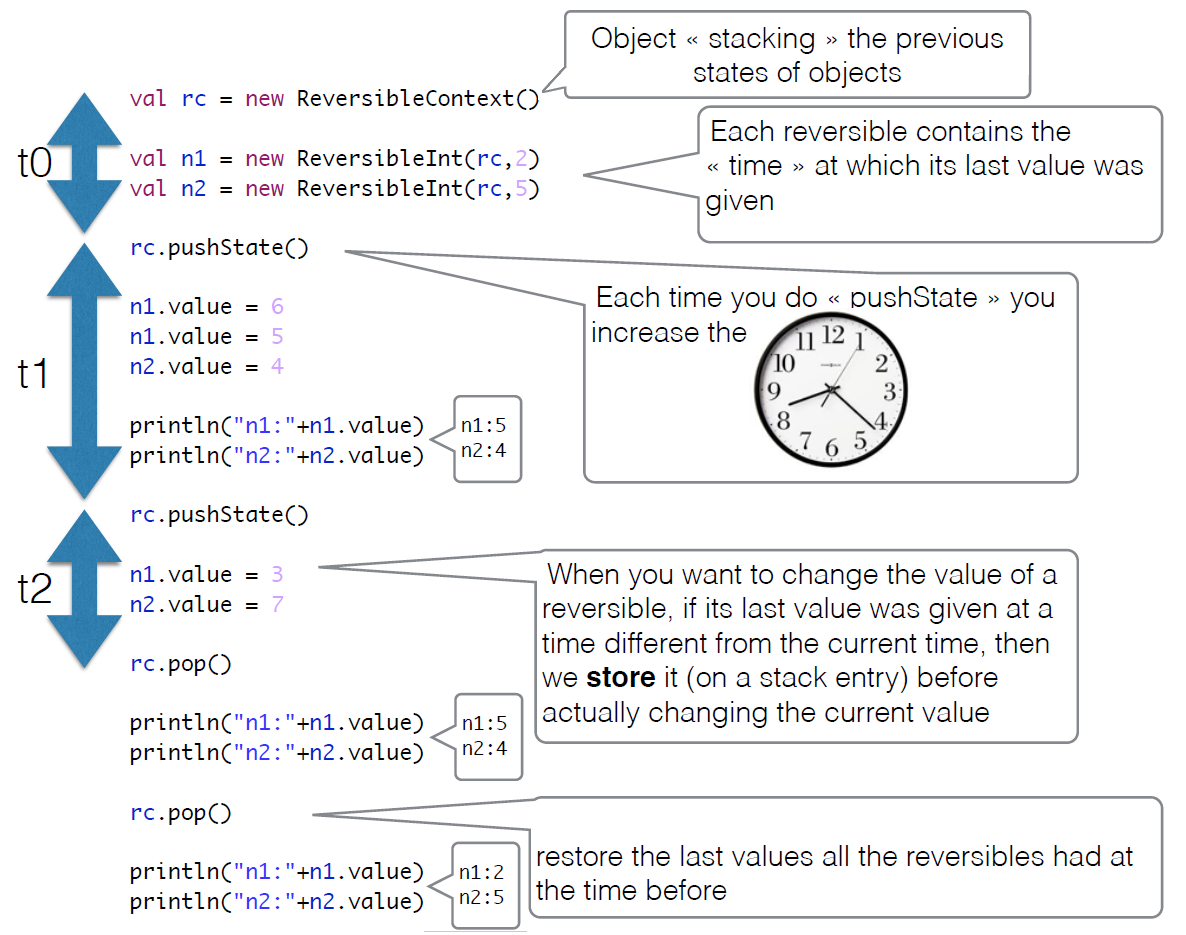
\includegraphics[width=\linewidth]{ReversibleIntegerIntroductionBB.png}
    \label{fig:Knapsack_example}
\end{figure}
\FloatBarrier

With the push pop operation acting as follows:

\begin{figure}[!ht]
    \centering
    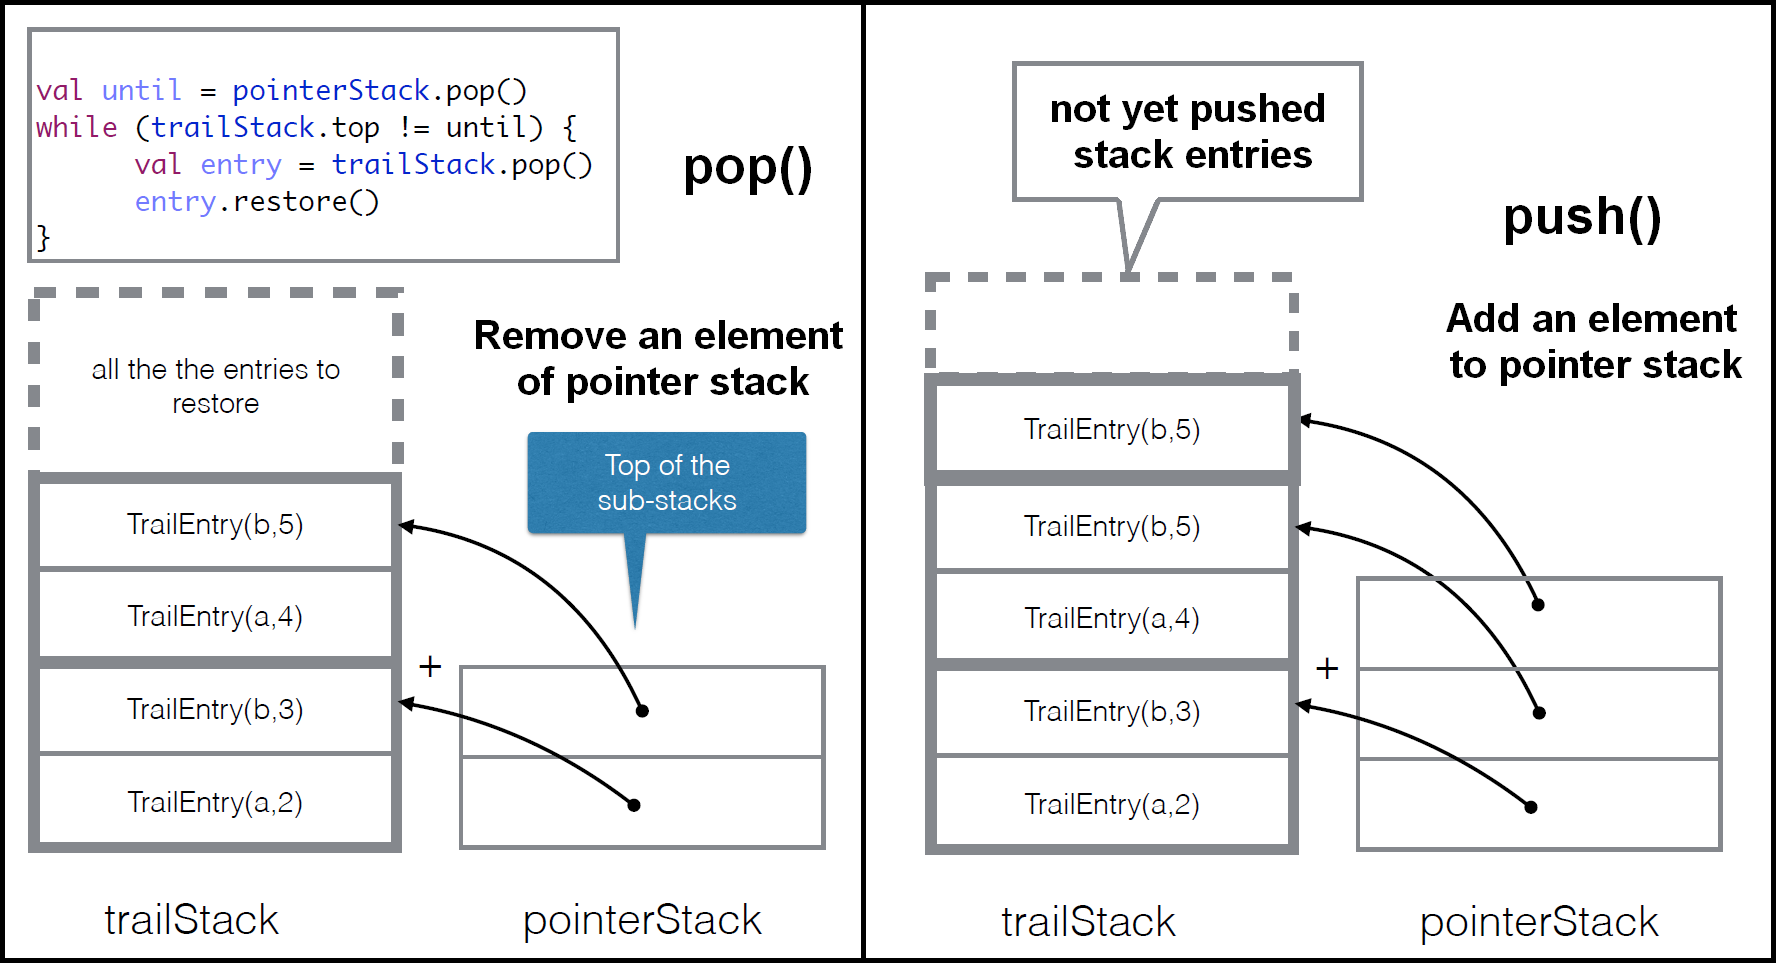
\includegraphics[width=0.9\linewidth]{ReversibleStatePushPop.png}
    \caption{Push/Pop implementation in reversible context}
    \label{fig:Knapsack_example}
\end{figure}
\FloatBarrier

\subsubsection{Implementation}

\#Ca pue l'exam les gars

\begin{figure}[!ht]
    \centering
    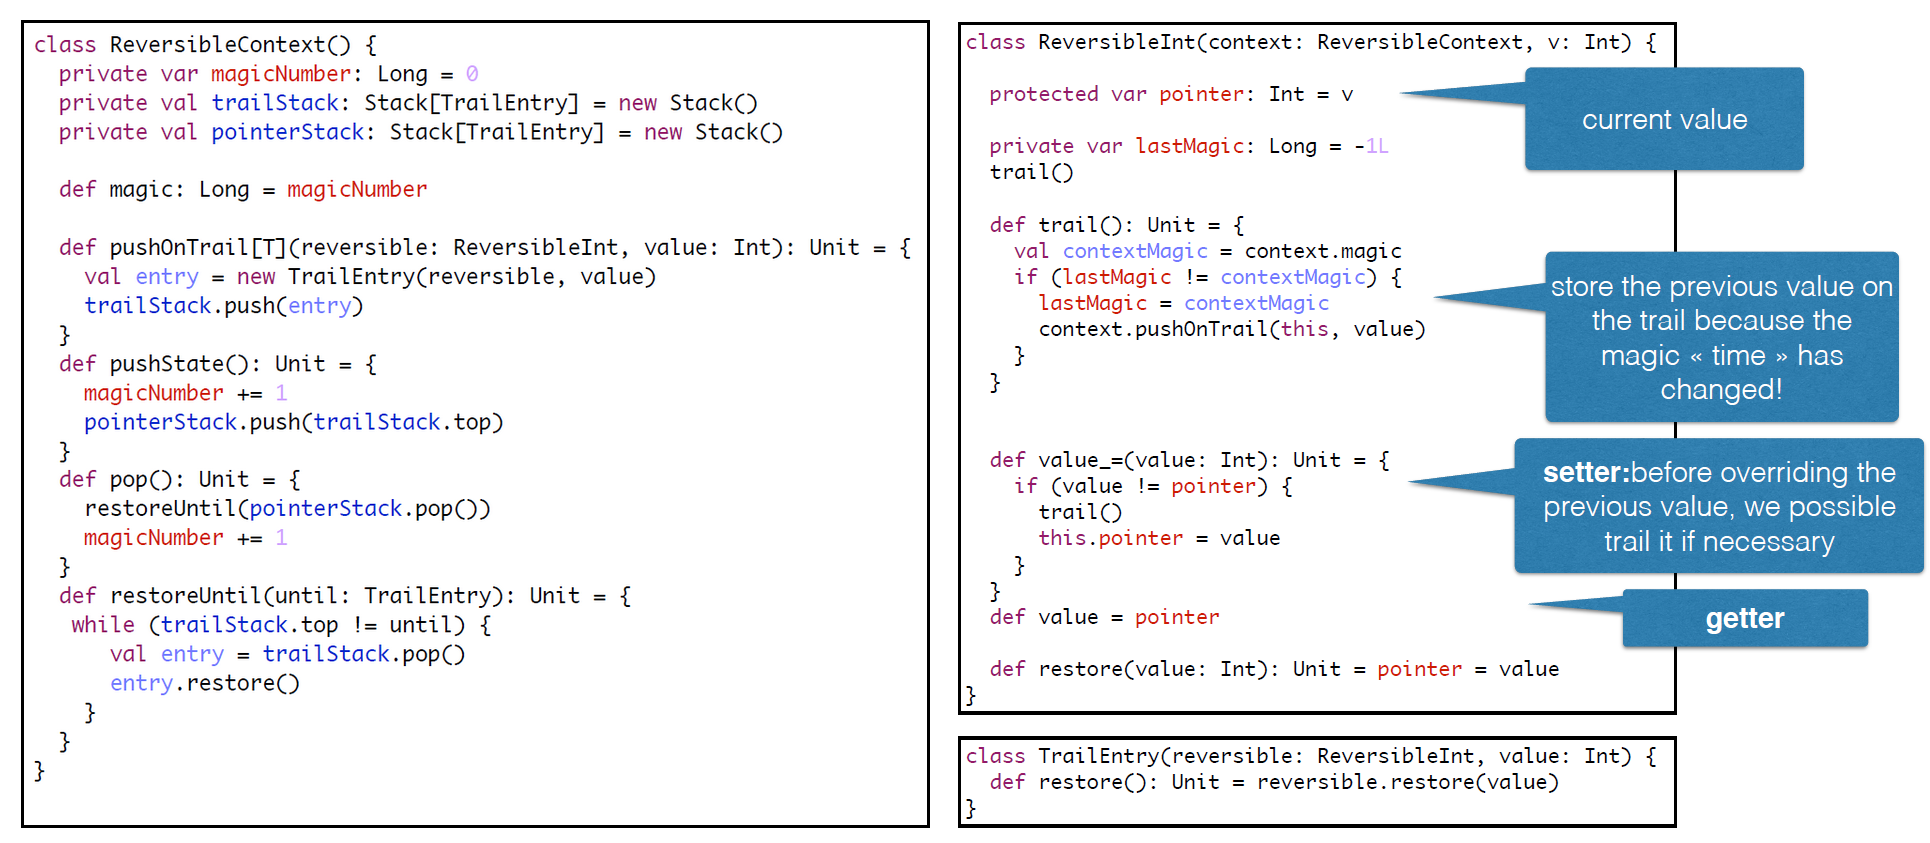
\includegraphics[width=1.1\linewidth]{ReversibleStateImplementation.png}
    \label{fig:Knapsack_example}
\end{figure}
\FloatBarrier

The slides (lecture 2 page 28) contains an implementation of B\&B using branch and bound
which we will not place here as it is highly unlikely that we will be interrogated on it.
Also if you have understood reversible context then it should be fairly easy 
to reimplement in the worst case scenario.

\subsection{Search heuristics}

So far we have always added items on the left side of the tree (affecting variable to 1)
and removed items on the right side. We have also always affected variable sequentially, 
in the same order each time\newline

Now that we can traverse the tree as we want, we can change that and make use of 
heuristics which, at each given moment, decide what variable to instantiate 
and/or which value to assign. 
\newline

In a Branch and bound algorithm, finding good solution faster is better 
as the pruning will become more effective.
Heuristic will also result in a better \textbf{anytime behavior} (the quality of the best
solution you have if you stop the search after a time limit).  \newline

\subsubsection{Iterative Discrepancy Search}

Discrepancy = Number of right (the side in a tree) decisions

If i posses a trustworthy heuristic where interesting sub tree are on the left of a parent,
using a limited discrepancy search would be a good optimisation as wrong decision often
take place in early stages.

\begin{figure}[!ht]
    \centering
    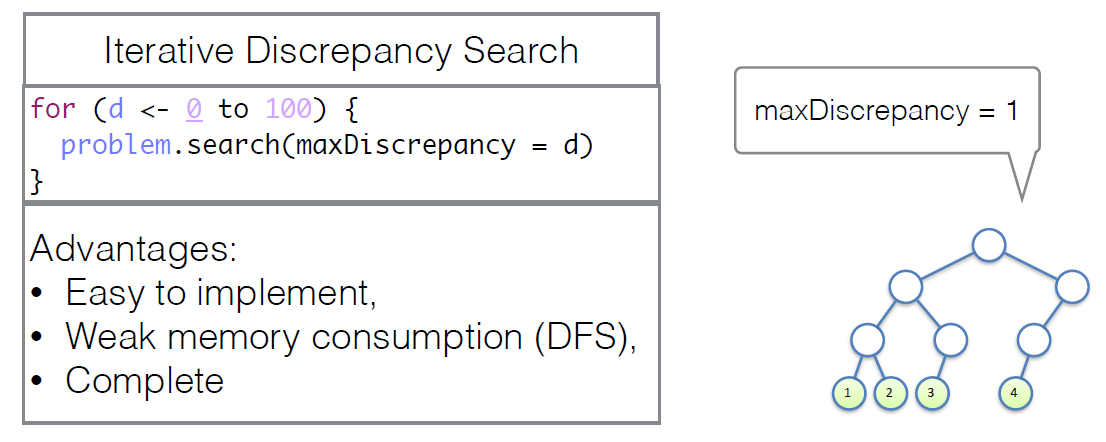
\includegraphics[width=0.8\linewidth]{LimitedDiscrepancySearch.png}
    \label{fig:Knapsack_example}
\end{figure}
\FloatBarrier

As you can see with this method we rapidly find good solution which will help the pruning
during the following iterations. We thus obtain a potentially fast and complete algorithm
(depending on the heuristic). If the heuristic is not significant however the algorithm will
be far slower as it involves much re computation (which normally won't be too signifiant
thanks to the pruning).\newline

\textbf{If the discrepancy search does not explore the tree completely, 
it is not considered complete !} This can however be used as a form of greedy
algorithm.

\subsubsection{Best first search}

Expand the open node with the best upper-bound first (maximization) !
Although fairly efficient and easy to implement, this heuristic has two drawbacks :

\begin{enumerate}
	\item You won't have a feasible solution directly (implication for the pruning).
	\item Memory usage is difficult to control.
\end{enumerate}

\begin{figure}[!ht]
    \centering
    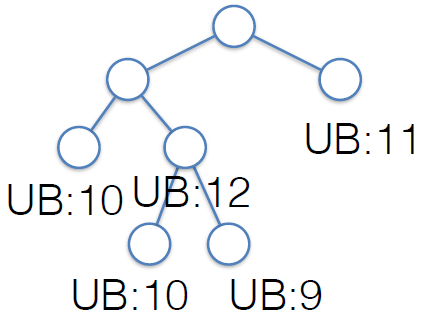
\includegraphics[width=0.3\linewidth]{BestFirstSearchBBHeuristic.png}
    \caption{Representation of the best first search heuristic}
    \label{fig:Knapsack_example}
\end{figure}
\FloatBarrier

\subsubsection{Other heuristics}

TODO

\subsection{Other B\&B optimisations}

\subsubsection{Symmetry detection}

In case of symmetric items in the knapsack set (understand identical), we can reduce the
search space significantly as the items are completely interchangeable.\newline

For example given four symmetrical items $(X_{n+1}, X_{n+2}, X_{n+3}, X_{n+4})$, 
their assignment tree would normally contain 16 elements $(2^4)$ but it can 
be reduced to five due to their symmetrical property. 
We only need to explore the following states:

\begin{enumerate}
	\item (0,0,0,0) => take 0
	\item (1,0,0,0) => take 1
	\item (1,1,0,0) => take 2
	\item (1,1,1,0) => take 3
	\item (1,1,1,1) => take 4
\end{enumerate}

\subsubsection{Dominance detection}

In case an item b is dominated by another item a
(b is dominated by a if $V_a \geq V_b \wedge W_a \leq W_b$)
It is never interesting to take b if a is not also taken ! \newline

An optimal solution cannot have a = 0 and b = 1. 
We can thus avoid to explore such states.

\subsection{Bonus questions and exam questions}

\subsubsection{Reversible set}

\begin{lstlisting}
//WARNING : UNTESTED but the idea is there

//Create ReversibleSet class as follows
// 1 : Add set variable which store curent set
// 2 : Modify pointer to save multiples changes
// 3 : Add remove method which remove in set and adds to changes made
// 4 : Modify trail method to push changes one by one
// 5 : Modifify restore methode to remove unpushed changes and add back argument value
// 6 : Write the get iterator method

class ReversibleSet(context: ReversibleContext, s: Set) {
	protected var currentSet: Set = s //Set
	protected var pointer: Array<Integer> = [] //List of changes
	private var lastMagic: Long = -1L
	trail()
	
	def trail(): Unit = {
		val contextMagic = context.magic
		if (lastMagic != contextMagic) {
			//We need to push values
			lastMagic = contextMagic
			for elem in pointer{ //One push per elem removed
				context.pushOnTrail(this, elem)
			}
			pointer = [] //Reset change array since change have been pushed
		}
	}
	def remove(value: Int): Unit = {
		if (value != pointer) {
			trail() //Always call this method before making changes
			this.currentSet.remove(value) //Remove value in set
			this.pointer.add(value) //Add to changes made
		}
	}
	def getIterator() : Unit = {
		return set.iterator(); //Assuming our set implements iterable
	}
	def set = currentSet //To acces current set value
	
	def restore(value: Int): Unit = {
		//Remove unpushed changes
		for elem in value{
			set.add(elem)
		}
		//(so that we don't add multiple time in case of multiple changes)
		pointer = [] //Reinit change list 
		//Add the value in argument to the set
		set.add(value);
	}
}
\end{lstlisting}

\subsubsection{Explicit stack DFS's pseudo code}

\begin{lstlisting}
//Init stack
stack state_to_visit = new stack();
state_to_visit.add((0,initState)); 
//A tuple (current index, state where no item are taken)
//Init method variable
int maxIndex = nbVariableToAsssign - 1;
state bestSol = initState;
while(!state_to_visit.isEmpty()) {
  (index, state) = state_to_visit.pop();
  if(index > maxIndex){
  	//Computation finished, evaluate state
  	if(bestSol.value < state.value) bestSol = state;
  }
  else if(state.getUpperBound() > bestSol.value){
  	newState = state.makeCopy()
  	//Add current elem not selected state to stack
  	state_to_visit.push((index+1, state));
  	//Add current elem selected state to stack => will be visited first
  	newState.changeElemAtIndex(index, 1); //Set as taken
  	if(newState.isUnderCapacityConstraint()) state_to_visit.push((index+1, newState));
  }
}
return bestSol; 
\end{lstlisting}

